%% bare_jrnl_compsoc.tex
%% V1.4b
%% 2015/08/26
%% by Michael Shell
%% See:
%% http://www.michaelshell.org/
%% for current contact information.
%%
%% This is a skeleton file demonstrating the use of IEEEtran.cls
%% (requires IEEEtran.cls version 1.8b or later) with an IEEE
%% Computer Society journal paper.
%%
%% Support sites:
%% http://www.michaelshell.org/tex/ieeetran/
%% http://www.ctan.org/pkg/ieeetran
%% and
%% http://www.ieee.org/

%%*************************************************************************
%% Legal Notice:
%% This code is offered as-is without any warranty either expressed or
%% implied; without even the implied warranty of MERCHANTABILITY or
%% FITNESS FOR A PARTICULAR PURPOSE! 
%% User assumes all risk.
%% In no event shall the IEEE or any contributor to this code be liable for
%% any damages or losses, including, but not limited to, incidental,
%% consequential, or any other damages, resulting from the use or misuse
%% of any information contained here.
%%
%% All comments are the opinions of their respective authors and are not
%% necessarily endorsed by the IEEE.
%%
%% This work is distributed under the LaTeX Project Public License (LPPL)
%% ( http://www.latex-project.org/ ) version 1.3, and may be freely used,
%% distributed and modified. A copy of the LPPL, version 1.3, is included
%% in the base LaTeX documentation of all distributions of LaTeX released
%% 2003/12/01 or later.
%% Retain all contribution notices and credits.
%% ** Modified files should be clearly indicated as such, including  **
%% ** renaming them and changing author support contact information. **
%%*************************************************************************


% *** Authors should verify (and, if needed, correct) their LaTeX system  ***
% *** with the testflow diagnostic prior to trusting their LaTeX platform ***
% *** with production work. The IEEE's font choices and paper sizes can   ***
% *** trigger bugs that do not appear when using other class files.       ***                          ***
% The testflow support page is at:
% http://www.michaelshell.org/tex/testflow/

\documentclass[compsoc,journal,letterpaper,10pt,draftclsnofoot,onecolumn]{IEEEtran}
%
% If IEEEtran.cls has not been installed into the LaTeX system files,
% manually specify the path to it like:
% \documentclass[10pt,journal,compsoc]{../sty/IEEEtran}


% *** MISC UTILITY PACKAGES ***
%
%\usepackage{ifpdf}
% Heiko Oberdiek's ifpdf.sty is very useful if you need conditional
% compilation based on whether the output is pdf or dvi.
% usage:
% \ifpdf
%   % pdf code
% \else
%   % dvi code
% \fi
% The latest version of ifpdf.sty can be obtained from:
% http://www.ctan.org/pkg/ifpdf
% Also, note that IEEEtran.cls V1.7 and later provides a builtin
% \ifCLASSINFOpdf conditional that works the same way.
% When switching from latex to pdflatex and vice-versa, the compiler may
% have to be run twice to clear warning/error messages.






% *** CITATION PACKAGES ***
%
\ifCLASSOPTIONcompsoc
  % IEEE Computer Society needs nocompress option
  % requires cite.sty v4.0 or later (November 2003)
  \usepackage[nocompress]{cite}
\else
  % normal IEEE
  \usepackage{cite}
\fi
% cite.sty was written by Donald Arseneau
% V1.6 and later of IEEEtran pre-defines the format of the cite.sty package
% \cite{} output to follow that of the IEEE. Loading the cite package will
% result in citation numbers being automatically sorted and properly
% "compressed/ranged". e.g., [1], [9], [2], [7], [5], [6] without using
% cite.sty will become [1], [2], [5]--[7], [9] using cite.sty. cite.sty's
% \cite will automatically add leading space, if needed. Use cite.sty's
% noadjust option (cite.sty V3.8 and later) if you want to turn this off
% such as if a citation ever needs to be enclosed in parenthesis.
% cite.sty is already installed on most LaTeX systems. Be sure and use
% version 5.0 (2009-03-20) and later if using hyperref.sty.
% The latest version can be obtained at:
% http://www.ctan.org/pkg/cite
% The documentation is contained in the cite.sty file itself.
%
% Note that some packages require special options to format as the Computer
% Society requires. In particular, Computer Society  papers do not use
% compressed citation ranges as is done in typical IEEE papers
% (e.g., [1]-[4]). Instead, they list every citation separately in order
% (e.g., [1], [2], [3], [4]). To get the latter we need to load the cite
% package with the nocompress option which is supported by cite.sty v4.0
% and later. Note also the use of a CLASSOPTION conditional provided by
% IEEEtran.cls V1.7 and later.





% *** GRAPHICS RELATED PACKAGES ***
%
\ifCLASSINFOpdf
   \usepackage[pdftex]{graphicx}
  % declare the path(s) where your graphic files are
   \graphicspath{{../media/}}
  % and their extensions so you won't have to specify these with
  % every instance of \includegraphics
  \DeclareGraphicsExtensions{.pdf,.jpeg,.png}
\else
  % or other class option (dvipsone, dvipdf, if not using dvips). graphicx
  % will default to the driver specified in the system graphics.cfg if no
  % driver is specified.
  \usepackage[dvips]{graphicx}
  % declare the path(s) where your graphic files are
  \graphicspath{{../media/}}
  % and their extensions so you won't have to specify these with
  % every instance of \includegraphics
  \DeclareGraphicsExtensions{.eps}
\fi
% graphicx was written by David Carlisle and Sebastian Rahtz. It is
% required if you want graphics, photos, etc. graphicx.sty is already
% installed on most LaTeX systems. The latest version and documentation
% can be obtained at: 
% http://www.ctan.org/pkg/graphicx
% Another good source of documentation is "Using Imported Graphics in
% LaTeX2e" by Keith Reckdahl which can be found at:
% http://www.ctan.org/pkg/epslatex
%
% latex, and pdflatex in dvi mode, support graphics in encapsulated
% postscript (.eps) format. pdflatex in pdf mode supports graphics
% in .pdf, .jpeg, .png and .mps (metapost) formats. Users should ensure
% that all non-photo figures use a vector format (.eps, .pdf, .mps) and
% not a bitmapped formats (.jpeg, .png). The IEEE frowns on bitmapped formats
% which can result in "jaggedy"/blurry rendering of lines and letters as
% well as large increases in file sizes.
%
% You can find documentation about the pdfTeX application at:
% http://www.tug.org/applications/pdftex






% *** MATH PACKAGES ***
%
\usepackage{amsmath}
% A popular package from the American Mathematical Society that provides
% many useful and powerful commands for dealing with mathematics.
%
% Note that the amsmath package sets \interdisplaylinepenalty to 10000
% thus preventing page breaks from occurring within multiline equations. Use:
\interdisplaylinepenalty=2500
% after loading amsmath to restore such page breaks as IEEEtran.cls normally
% does. amsmath.sty is already installed on most LaTeX systems. The latest
% version and documentation can be obtained at:
% http://www.ctan.org/pkg/amsmath

\usepackage{amssymb}



% *** SPECIALIZED LIST PACKAGES ***
%
%\usepackage{algorithmic}
% algorithmic.sty was written by Peter Williams and Rogerio Brito.
% This package provides an algorithmic environment fo describing algorithms.
% You can use the algorithmic environment in-text or within a figure
% environment to provide for a floating algorithm. Do NOT use the algorithm
% floating environment provided by algorithm.sty (by the same authors) or
% algorithm2e.sty (by Christophe Fiorio) as the IEEE does not use dedicated
% algorithm float types and packages that provide these will not provide
% correct IEEE style captions. The latest version and documentation of
% algorithmic.sty can be obtained at:
% http://www.ctan.org/pkg/algorithms
% Also of interest may be the (relatively newer and more customizable)
% algorithmicx.sty package by Szasz Janos:
% http://www.ctan.org/pkg/algorithmicx




% *** ALIGNMENT PACKAGES ***
%
\usepackage{array}
% Frank Mittelbach's and David Carlisle's array.sty patches and improves
% the standard LaTeX2e array and tabular environments to provide better
% appearance and additional user controls. As the default LaTeX2e table
% generation code is lacking to the point of almost being broken with
% respect to the quality of the end results, all users are strongly
% advised to use an enhanced (at the very least that provided by array.sty)
% set of table tools. array.sty is already installed on most systems. The
% latest version and documentation can be obtained at:
% http://www.ctan.org/pkg/array


% IEEEtran contains the IEEEeqnarray family of commands that can be used to
% generate multiline equations as well as matrices, tables, etc., of high
% quality.




% *** SUBFIGURE PACKAGES ***
\ifCLASSOPTIONcompsoc
  \usepackage[caption=false,font=footnotesize,labelfont=sf,textfont=sf]{subfig}
\else
  \usepackage[caption=false,font=footnotesize]{subfig}
\fi
% subfig.sty, written by Steven Douglas Cochran, is the modern replacement
% for subfigure.sty, the latter of which is no longer maintained and is
% incompatible with some LaTeX packages including fixltx2e. However,
% subfig.sty requires and automatically loads Axel Sommerfeldt's caption.sty
% which will override IEEEtran.cls' handling of captions and this will result
% in non-IEEE style figure/table captions. To prevent this problem, be sure
% and invoke subfig.sty's "caption=false" package option (available since
% subfig.sty version 1.3, 2005/06/28) as this is will preserve IEEEtran.cls
% handling of captions.
% Note that the Computer Society format requires a sans serif font rather
% than the serif font used in traditional IEEE formatting and thus the need
% to invoke different subfig.sty package options depending on whether
% compsoc mode has been enabled.
%
% The latest version and documentation of subfig.sty can be obtained at:
% http://www.ctan.org/pkg/subfig




% *** FLOAT PACKAGES ***
%
\usepackage{fixltx2e}
% fixltx2e, the successor to the earlier fix2col.sty, was written by
% Frank Mittelbach and David Carlisle. This package corrects a few problems
% in the LaTeX2e kernel, the most notable of which is that in current
% LaTeX2e releases, the ordering of single and double column floats is not
% guaranteed to be preserved. Thus, an unpatched LaTeX2e can allow a
% single column figure to be placed prior to an earlier double column
% figure.
% Be aware that LaTeX2e kernels dated 2015 and later have fixltx2e.sty's
% corrections already built into the system in which case a warning will
% be issued if an attempt is made to load fixltx2e.sty as it is no longer
% needed.
% The latest version and documentation can be found at:
% http://www.ctan.org/pkg/fixltx2e


%\usepackage{stfloats}
% stfloats.sty was written by Sigitas Tolusis. This package gives LaTeX2e
% the ability to do double column floats at the bottom of the page as well
% as the top. (e.g., "\begin{figure*}[!b]" is not normally possible in
% LaTeX2e). It also provides a command:
%\fnbelowfloat
% to enable the placement of footnotes below bottom floats (the standard
% LaTeX2e kernel puts them above bottom floats). This is an invasive package
% which rewrites many portions of the LaTeX2e float routines. It may not work
% with other packages that modify the LaTeX2e float routines. The latest
% version and documentation can be obtained at:
% http://www.ctan.org/pkg/stfloats
% Do not use the stfloats baselinefloat ability as the IEEE does not allow
% \baselineskip to stretch. Authors submitting work to the IEEE should note
% that the IEEE rarely uses double column equations and that authors should try
% to avoid such use. Do not be tempted to use the cuted.sty or midfloat.sty
% packages (also by Sigitas Tolusis) as the IEEE does not format its papers in
% such ways.
% Do not attempt to use stfloats with fixltx2e as they are incompatible.
% Instead, use Morten Hogholm'a dblfloatfix which combines the features
% of both fixltx2e and stfloats:
%
% \usepackage{dblfloatfix}
% The latest version can be found at:
% http://www.ctan.org/pkg/dblfloatfix




%\ifCLASSOPTIONcaptionsoff
%  \usepackage[nomarkers]{endfloat}
% \let\MYoriglatexcaption\caption
% \renewcommand{\caption}[2][\relax]{\MYoriglatexcaption[#2]{#2}}
%\fi
% endfloat.sty was written by James Darrell McCauley, Jeff Goldberg and 
% Axel Sommerfeldt. This package may be useful when used in conjunction with 
% IEEEtran.cls'  captionsoff option. Some IEEE journals/societies require that
% submissions have lists of figures/tables at the end of the paper and that
% figures/tables without any captions are placed on a page by themselves at
% the end of the document. If needed, the draftcls IEEEtran class option or
% \CLASSINPUTbaselinestretch interface can be used to increase the line
% spacing as well. Be sure and use the nomarkers option of endfloat to
% prevent endfloat from "marking" where the figures would have been placed
% in the text. The two hack lines of code above are a slight modification of
% that suggested by in the endfloat docs (section 8.4.1) to ensure that
% the full captions always appear in the list of figures/tables - even if
% the user used the short optional argument of \caption[]{}.
% IEEE papers do not typically make use of \caption[]'s optional argument,
% so this should not be an issue. A similar trick can be used to disable
% captions of packages such as subfig.sty that lack options to turn off
% the subcaptions:
% For subfig.sty:
% \let\MYorigsubfloat\subfloat
% \renewcommand{\subfloat}[2][\relax]{\MYorigsubfloat[]{#2}}
% However, the above trick will not work if both optional arguments of
% the \subfloat command are used. Furthermore, there needs to be a
% description of each subfigure *somewhere* and endfloat does not add
% subfigure captions to its list of figures. Thus, the best approach is to
% avoid the use of subfigure captions (many IEEE journals avoid them anyway)
% and instead reference/explain all the subfigures within the main caption.
% The latest version of endfloat.sty and its documentation can obtained at:
% http://www.ctan.org/pkg/endfloat
%
% The IEEEtran \ifCLASSOPTIONcaptionsoff conditional can also be used
% later in the document, say, to conditionally put the References on a 
% page by themselves.




% *** PDF, URL AND HYPERLINK PACKAGES ***
%
%\usepackage{url}
% url.sty was written by Donald Arseneau. It provides better support for
% handling and breaking URLs. url.sty is already installed on most LaTeX
% systems. The latest version and documentation can be obtained at:
% http://www.ctan.org/pkg/url
% Basically, \url{my_url_here}.





% *** Do not adjust lengths that control margins, column widths, etc. ***
% *** Do not use packages that alter fonts (such as pslatex).         ***
% There should be no need to do such things with IEEEtran.cls V1.6 and later.
% (Unless specifically asked to do so by the journal or conference you plan
% to submit to, of course. )








%\usepackage{lmodern}
%\usepackage{amssymb,amsmath}
%\usepackage{ifxetex,ifluatex}
%\usepackage{fixltx2e} % provides \textsubscript
%\ifnum 0\ifxetex 1\fi\ifluatex 1\fi=0 % if pdftex
%  \usepackage[T1]{fontenc}
%  \usepackage[utf8]{inputenc}
%\else % if luatex or xelatex
% \ifxetex
%  \usepackage{mathspec}
%  \else
%   \usepackage{fontspec}
%  \fi
%\fi
%\usepackage[unicode=true]{hyperref}
%\hypersetup{
%           pdfborder={0 0 0},
%           breaklinks=true}
%\urlstyle{same}  % don't use monospace font for urls
%\usepackage{longtable,booktabs}
%% Fix footnotes in tables (requires footnote package)
%\IfFileExists{footnote.sty}{\usepackage{footnote}\makesavenoteenv{long table}}{}
%\usepackage{graphicx,grffile}
%\makeatletter
%\def\maxwidth{\ifdim\Gin@nat@width>\linewidth\linewidth\else\Gin@nat@width\fi}
%\def\maxheight{\ifdim\Gin@nat@height>\textheight\textheight\else\Gin@nat@height\fi}
%\makeatother
%% Scale images if necessary, so that they will not overflow the page
%% margins by default, and it is still possible to overwrite the defaults
%% using explicit options in \includegraphics[width, height, ...]{}
%\setkeys{Gin}{width=\maxwidth,height=\maxheight,keepaspectratio}
%\IfFileExists{parskip.sty}{%
%\usepackage{parskip}
%}{% else
%\setlength{\parindent}{0pt}
%\setlength{\parskip}{6pt plus 2pt minus 1pt}
%}
%\setlength{\emergencystretch}{3em}  % prevent overfull lines
%\providecommand{\tightlist}{%
%  \setlength{\itemsep}{0pt}\setlength{\parskip}{0pt}}
%\setcounter{secnumdepth}{0}
%% Redefines (sub)paragraphs to behave more like sections
%\ifx\paragraph\undefined\else
%\let\oldparagraph\paragraph
%\renewcommand{\paragraph}[1]{\oldparagraph{#1}\mbox{}}
%\fi
%\ifx\subparagraph\undefined\else
%\let\oldsubparagraph\subparagraph
%\renewcommand{\subparagraph}[1]{\oldsubparagraph{#1}\mbox{}}
%\fi

%% set default figure placement to htbp
%\makeatletter
%\def\fps@figure{htbp}
%\makeatother




%%%%%
%%%%%                                         Our definitions
%%%%%

\DeclareMathOperator*{\argmax}{arg\,max}

%%%%%
%%%%%
%%%%%

\date{\today}

\begin{document}

\begin{abstract}
Optimal behaviour policies for non-degenerate Markov Decision Processes
(nMDPs) can be intractable to find, when state space size is
prohibitive. In this paper, a theoretical method of deconstruction nMDPs
into a set of concurrent MDPs is demonstrated. Such concurrent
representations may be degenerate in state space, and require
exponentially less memory to store. In offset of the state space
savings, it frequently believed that such degeneracies lead to
sub-optimal policy regression. Surprisingly, given weak preconditions,
policy regression for the degenerate Concurrent MDP sets (CMDP) can
converge upon optimal policies for the coincident non-degenerate nMDPs.
To illustrate this effect a theoretical exploration is followed by a
simple localization and box pushing simulation. In validation of the
position, regression approaches using Q-Learning did not yield
statistically significant behaviour policies in terms of reward
maximization, despite the fact that the degenerate CMDP required
exponentially less state space to specify (pairwise p-value \textless{}
X.XXXX ).
\end{abstract}

\section{Introduction}\label{introduction}

In prior work Concurrent Markov Decision Processes were presented
{[}{]}, and shown via experiment to enable discovery locally policy when
compared with nMDPs. Among some theoretical questions, the question of
how a set of degenerate MDPs, with partial state spaces, could converge
on identical or superior policies as compared with the non-degenerate
MDP was left as future work. Indeed, for people, we routinely choose to
represent partial truths to ourselves, or give attention to subsets of
our sensory information, such that our daily tasks are simplified. Thus,
future intelligent agents, including robots, may need to rely on similar
coping mechanisms that broadly introduce state degeneracy into problem
models for the sake of efficiency. The work on CMDPs demonstrated that
this approach, of introducing state degeneracy, may have theoretical
merits. This paper grounds the state degeneracy discovery in theory.

This paper exposes and explores some weak problem assumptions that are
made when performing a split of a non-degenerate MDP into a set of
Concurrent Markov Decision Processes. When these weak assumptions are
met, it is demonstrated that identical or superior local policy
regression is expected both theoretically and empirically. Thus, this
work contributes this set of assumptions which may be validated when
simplifying nMDP problems into CMDP problems.

This paper outlines a brief background related to state space
representation in Section 1, before outlining the core CMDP theory in
Section 2. Section 3 outlines how a simple version of Q-Learning can be
used to contrast the state space representation experiment. In Section
4, results are demonstrated for a simple localization and box pushing
experiment.

\section{Background}\label{background}

The idea of state space factorization is not novel, and falls broadly
into three categories.

In all approaches, it is frequently assumed in the literature that
models which are degenerate in state space will expectedly suffer in the
quality of their local optima. Broadly speaking, in Machine Learning
literature, this is sometimes expressed as the Bias-Variance trade off.
Practically speaking, when creating degenerate MDPs, the question of
\emph{how degenerate} these MDPs may be until they become biased is
sometimes considered to be a core question.

Thus in this paper we present a method, given what is believed to be a
non-degenerate and intractable nMDP, to construct and converge on an
optimal behaviour policy. The method includes splitting the nMDP into a
tractable CMDP form. We demonstrate both analytically and empirically,
that the regressed policies are identical in terms of local optimality,
if certain conditions hold.

\section{Theory}\label{theory}

First, it is shown that an nMDP can be split into sub dependent MDPs,
denoted a CMDP. Afterwards a lemma is provided which may be reused when
approaching nMDP deconstruction.

\subsection{Definitions, Concurrent Markov Decision
Processes}\label{definitions-concurrent-markov-decision-processes}

To begin MDP problem definition, we broadly consider the task of finding
the optimal location in a discrete state space in
\(S = \mathbb{N}^{N}\), using the maximum value function
\(V:S\rightarrow\mathbb{R}\). To ensure the space \(S\) has an
optimal element it is assumed that a certain rearrangement of the value
image \(V\left( S \right)\) monotonic.

Thus, to discover a solution to the problem, the help of an agent may be
elicited, who has allowed actions in a set \(A \subset \mathbb{N}\), for
every instant \(t \in \mathbf{T}\subset\mathbb{N}\). The
convention that an agent chooses an action \(a_{t} \in A\) for every
state \(s_{t} \in S\), before arriving in state \(s_{t + 1} \in S\) is
followed. The probability \(T\left( s_{t + 1} |s_{t}, a_{t}\right)\)
represents the true and observed transitional probability of the system,
also described as the dynamics of the environment, which are assumed to
be stably stochastic, unless started otherwise. The epoch \(E_{e}\)is a
set of contiguous time indexes, with restrictions:
\(e_{i}\in\mathbb{N}\), \(\bigcup_{e = 1}^{\mathbb{N}}E_{e} = \mathbf{T}\), and
\(\bigcup_{e_{1},e_{2}\in\mathbb{ N}}{E_{e_{1}} \cap E_{e_{2}}} = \{\varnothing\}\).
We assume the size of the epochs increase
\(\left| e_{i} \right| < \left| e_{(i + 1)} \right|\), meaning that
over time more time instants are contained within each. It is assumed
that some discoverable infinite horizon reward exists
\(R\left( s_{t}, a_{t}, s_{t + 1} \right)\) such that agents may attempt
to ``maximize'' the value given by the trajectory, where the value of a
state is given by \(V\left( S \right).\)

\begin{equation}
V\left( s_{t} \right) = \sum_{s_{t + 1} \in S\ }{P\left( s_{t + 1}|s_{t},a_{t} \right)\left( R\left( s_{t},a_{t},s_{t + 1} \right) + \gamma V\left( s_{t + 1} \right) \right)}
\end{equation}

The goal is to (a) explore and map the quality
\(Q_{t}:S \times A\mathbb{\rightarrow R}\) for the space, such that (b)
a behavioural policy \(a_{t} = \pi_{t}(s_{t}, a_{t})\) is partly
characterized by the \(Q_{t}\) values of the state. Commonly, the naive
optimal policy is given by \(\pi^{*}\):

\begin{equation}
\pi^{*}\left( s_{t} \right) \leftarrow \argmax_{a}{Q_{t}(s_{t},a)} 
\end{equation}

The above MDP definition is frequently expressed as a tuple:
\(m_{k} = \langle S_{k}, A_{k}, T_{k}, R_{k}, \pi_{k} \rangle\), where the initial posed
nMDP problem is noted as
\(m = \langle S, A, T, R,\pi \rangle \). The time index
\(t\), may sometimes be replaced with an epoch index \(e\), in
situations that an MDP \(m_{i}\)operates on a different discrete
timescale than another MDP \(m_{j}\).

\subsubsection{Random Field Deconstruction
Example}\label{random-field-deconstruction-example}

\begin{figure}
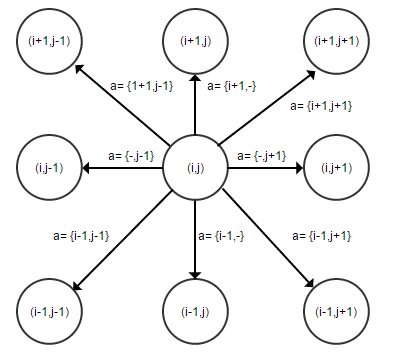
\includegraphics[width=2.68750in,height=2.80556in]{media/image1.png}\\
\caption{\label{fig:figure1}The nMDP with transitions from \((i,j)\)only.}
\end{figure}

The
problem of the random field with real values can be considered,
\(r:X^{N} \rightarrow \mathbb{R}^{+}\ \ ,\ X\mathbb{\subset N}\), which
we assume is well-ordered and monotonic. For brevity, we consider
\(N = 2\) as a visual example.

\paragraph{An nMDP definition can be
described}\label{an-nmdp-definition-can-be-described}

\begin{itemize}
\item
  \(S = X^{N}\) is the set of all possible states
\item
  \(A = A_{u} \times A_{l} \) \ s.t.\  \ 
  \( A_{u}, A_{l} = \left\{ - 1,1,\varnothing \right\}\)

  \begin{itemize}
  \item
    with \(a_{u} \in A_{u}, a_{l} \in A_{l}\)
  \end{itemize}
\item
  \(R\left( s_{t + 1}|s_{t}, a_{t} \right) = r\left( l + a_{l}, u + a_{u} \right) - r(l,u)\)
\item
  \(T\left( \left\{ l + a_{l},u + a_{u} \right\}|,\{ a_{l},a_{u}\},\{ l,u\} \right) = 1\),
  \(0\) otherwise

  In terms of notation the following equalities are always true:
  \(s_{t + 1} = \{ i + a_{u}, j + a_{l}\}\), \(a_{t} = \{ a_{u},a_{l}\}\), and\(\ s_{t} = \{ i,j\}\).
\end{itemize}

Thus, the problem for a reinforcement learning agent may be to localize
and converge upon an optimal space \(s_{t}\) such that \(r(s_{t})\) is
maximized. The agent can, without fail, move in any combination of
``up'', ``left'', ''down'', ''right'', and ``nothing'' to localize the
best location. A discount reward and infinite time horizon are
considered.

It turns out that the nMDP problem can be restated in terms of a
degenerate manner using two models with degenerate state space.
Colloquially, an agent can solve a degenerate CMDP problem of locating
the best column and row independently.

\subsubsection[An CMDP definition can be
described]{ An CMDP definition can be described}\label{an-cmdp-definition-can-be-described}

\begin{figure}
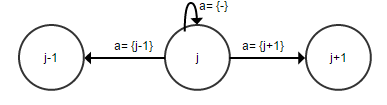
\includegraphics{media/image3.png}\\
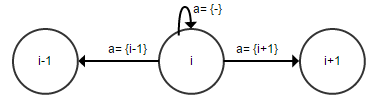
\includegraphics{media/image4.png}\\
\caption{\label{fig:figure2} Parent (a) and child (b) within the CMDP.}
\end{figure}

First, a \emph{child} dependent MDP is defined

\begin{itemize}
\item
  \(S_{l}  = X^{1}, j\)
\item
  \(A_{l}\)
\item
  \(R_{l}\left( l + a_{l}|a_{l},l,u \right) = r\left( l + a_{l}, u \right) - r(l,u)\)
\item
  \(T_{l}\left( l + a_{l}|a_{l}, l, \right) = 1, 0\) otherwise
\item
  The sequence index \(t\) is used for the child MDP.
\item
  \(M_{l} = \left\langle S_{l}, A_{l} ,T_{l}, R_{l} \right\rangle\)
\end{itemize}

Second, a \emph{parent} dependent MDP is defined

\begin{itemize}
\item
  \(S_{u}\  = X^{1},i\)
\item
  \(A_{u}\)
\item
  \(R_{u}\left( u + a_{u}|a_{u},u,E_{e} \right) = R_{u}\left( s_{u,e + 1}|a_{u,e},s_{u,e},E_{e} \right)\)

  \begin{itemize}
  \item
    Noting
    \(R_{u}\left( s_{u,e + 1}|a_{u,e}, s_{u,e}, E_{e} \right) = \sum_{t \in E_{e}}^{\ }\frac{R_{l}\left( s_{l,t + 1}|a_{l,t}, s_{l,t}, s_{u,t} \right)}{\overline{\overline E}_{e}} - \sum_{t \in E_{e}^{o}}^{\ }\frac{R_{l}\left( s_{l,t + 1}|a_{l,t},s_{l,t},s_{u,t} \right)}{\overline{\overline E}_{e}^{o}}\)
  \end{itemize}
\item
  \(T_{u}\left( u + a_{u}|a_{u}, u \right) = 1,\ 0\) otherwise
\item
  \(M_{u} = \left\langle S_{u}, A_{u}, T_{u}, R_{u} \right\rangle\)
\item
\item
  The sequence index \(e\) is used for the parent MDP.
\end{itemize}

For notation, the equalities are always true:
\(s_{x,t + 1} = x + a_{x}\), \(a_{x,t} = a_{x}\) ,
and\(s_{x,t} = x\),\(a_{x,t}\), where \(x \in \{ l,u\}\), where a time
index \(t\) is substituted with and epoch \(e\) for the parent MDP. The
notation \(\overline{\overline E}_{e}\) represents the cardinality of an epoch,
and is variable in \(\mathbf{T}\).

\begin{figure}
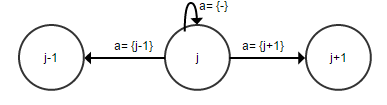
\includegraphics[width=3.20833in,height=1.70208in]{media/image3.png}\\
\caption{\label{fig:figure3}Block diagram of a CMDP.}
\end{figure}

Thus,
as mentioned in prior {[}{]},two MDPs can form an interdependent set,
such that the action \(a_{e}\) of the \emph{parent} MDP describes
reachable state space of a \emph{child} MDP, though restricting state
space exploration by defining variable \(u\). Conversely, the child
MDP's policy
\(\left\{ a_{t} = \pi_{t}(s_{t}) \right\}_{t \in E_{e}}^{\ }\) over all
timesteps defines the reward obtained
\(R_{u}\left( s_{e + 1}|a_{e},s_{e},E_{e} \right)\). A block diagram can
illustrate these dependencies.

\subsubsection{Policy Convergence}\label{policy-convergence}

We consider elementary q-learning: ELEMENTARY Q-LEARNING

In order for convergence to be ensured \(t \rightarrow \infty\), or
\(e \rightarrow \infty\), two conditions must be met: (a) an agent must
visit each state \(s \in S\) infinite times, (b) an agent's learning
rate \(\alpha\) must satisfy CONVERGENCE CRITERIA, and (c) the Reward
function and transitions probabilities \(T\), and \(R\) must be stably
stochastic.

A rudimentary action selection model \(\pi_{t}\ \)can involve sampling
the density function
\begin{equation}
\pi\left( s \right) \sim \left( s, a \right) = \frac{e^{Q_{t - 1}(s, a)}}{\sum_{b \in A}e^{Q_{t - 1}(s, b)}}
\end{equation}
Which can be shown to converge readily for an nMDP which satisfies the
three above conditions {[}{]}.

\subsubsection{Convergence}\label{convergence}

We now briefly show convergence of both the parent and child process
based on \(\pi_{t}\). Past interest, nothing is lost by moving to
section XXX. In general, optimal policies will be denoted
\(\pi^{*}(s) \in \Omega^{*}(s)\), where \(\Omega^{*}\) is the set of all
optimal policies, and the action selection policies \(\Omega^{*}(s)\)
represent the set of optimal action selection policies for a state
\(s \in \mathbf{S}\).

\paragraph{Child MDP Convergence on optimal
policy}\label{child-mdp-convergence-on-optimal-policy}

For the child MDP, it is clear that the epoch \(e \rightarrow \infty\)
duration increases as \(t \rightarrow \infty\). Thus we have:
\begin{align}
\lim_{e\rightarrow\infty}
\overline{\overline{E}}_{e} &= \infty \notag\\ 
\textrm{and}\qquad
\pi_{l}\left( s_{l}, a_{l} \right) &> 0
\end{align} 

We also know that, given all epoch \(e\),
\(\pi_{u}\left( s_{u},a_{u} \right) > 0\). Thus, all states are
reachable and infinite visitations at time infinity are assured. For a
sub space \(S_{l}\), for the child MDP, we note that the Q-Values
\(Q_{t}(s_{l},a_{l})\) will be reset to initialized values upon
transition to every new epoch \(e_{i + 1} \neq e_{i}\); in this case,
since \(\overline{\overline E}_{e} \rightarrow \infty\), we are assured that
policy convergence is possible. The practical problem of resetting the
Q-Values in a non-optimal way is addressed in the implementation
section, but in the worst case, (with resetting values,) eventual
convergence is theoretically assured.

\paragraph{Parent MDP Convergence on optimal
policy}\label{parent-mdp-convergence-on-optimal-policy}

Convergence for the parent MDP is apparent, as the reward function
\(R_{u}\left( s_{e + 1}|a_{e},s_{e},E_{e} \right)\) is not only stably
stochastic, but also increasingly reflective of the mean reward expected
from a learning agent given a target row \(j\). Since
\(\pi_{t}\left( s_{u},a_{u} \right) > 0\) and \(e \rightarrow \infty\),
with a stable transition model \(T_{u}\) convergence is assured.

\paragraph{Mapping Disjoint CMDP Policies onto an optimal nMDP
Policy}\label{mapping-disjoint-cmdp-policies-onto-an-optimal-nmdp-policy}

Having two convergent sub optimal policies (\(\pi_{u},\pi_{l}\)) is a
promising initial step, but may not contribute to the solution for an
optimal global policy \(\pi_{\ }.\) It turns out that it can under some
weak conditions, outlined below, such convergence can be shown readily.
Specifically we wish to map the set two sub optimal policies onto an
optimal nMDP policy:

\begin{equation}
f:\Omega_{u}^{*}\left( S_{u} \right) \times \Omega_{l}^{*}\left( S_{l} \right) \rightarrow \ {\tilde{\Omega}}^{*}\left( S \right):{\tilde{\Omega}}^{*}\left( S \right) \subseteq \Omega^{*}\left( S \right)
\end{equation}
 

For the above MDP problem, it can be readily demonstrated that such a
mapping function \(f\) can be found, given the above CMDP problem.
Specifically we must consider the nature of optimal policy for both the
parent and child MDPs. We begin with the definition of an optimal value
given a state \(s\):
\begin{equation}
\Omega^{*}(s) = \argmax_{a}\sum_{s' \in S}P\left( s'|s,a \right)\left( R\left( s, a, s' \right) + \gamma V\left( s' \right) \right)
\end{equation}
And, it follows directly that a specific and optimal global policy can
be expressed as every combination of optimal CMDP policies,
\(\pi^{*}\left( s \right) = \pi_{u}^{*}\left( s \right) \cup \pi_{l}^{*}\left( s \right)\).
For details on this detailed derivation, please see Convergent Factors
Lemma in the as the appendix. We also, then, know that execution of the
regular action policies will lead the Q-values to converge on these
optimal policies.
\begin{equation}
\pi\left( s \right) = \left\{ \pi_{u}\left( s \right),\pi_{l}\left( s \right) \right\}
\end{equation}

This technique can factor exponentially large state space problems into
polynomial space, rendering intractable problems as tractable. With the
addition a dynamic programming approach, the convergence speed can be
optimized, trading off storage space for convergence speed.

\subsubsection{Simulation}\label{simulation}

For simulation, we tackle the elementary two dimensional
\(S = X^{2}\), where \(X = \{ 1,2,\ldots,100\}\). Each cell is
assigned a valued
\(V\left( s \in S \right) \in \left\{ 1,\ldots,1000 \right\}\). We
contrast a nMDP approach, and its convergence time, with two CMDP
approaches, with all three described below.

\subsubsection{Example Derivation of multi-agent robotics
Application}\label{example-derivation-of-multi-agent-robotics-application}

After initial consideration of the nMDP problem, it can be illuminating
to consider how a multi-agent MDP can be expressed as a CMDP problem. In
general, when multi-agent MDPs are formed, they are approached from two
directions. Either the MDP representation is centralized, meaning that a
single nMDP contains all information across all agents, or each
individual agent possesses a subset of the compelte MDP problem,
sometimes called decentralized MDPs.

Decentralized MDPs commonly express degeneracy when compared with their
original problem. Importantly there has been work on decentralized MDPs
whose formulation allow seeming convergence on optimal solutions to
related nMDP problems. However, the theoretical accuracy of policy
convergence for multi-agent CMDP problems has been elusive.

Thus, the following derivation demonstrates how the general CMDP
approach can be used to derive a multi-agent CMDP for a mult-agent
robotics simulation, such that policy convergence for the multi-agent
CMDP can be identical to the intractable nMDP counterpart.

\subsubsection{Centralized nMDP}\label{centralized-nmdp}

The centralized nMDP is defined as a decentralized MDP that may consist
of a set of states \(S_{U}\) a set of system actions for each agent
\(A_{U} = \times_{i = 1}^{n}\left\{ A_{I} \cup A_{T} \right\}\), a real
valued reward function \(R_{U}\), and a stably stochastic transitional
model \(T_{U}\). The decentralized MDP is used in this paper as a
control to contrast with other learning models.

The value of the reward \(R_{T}\) and transition functions \(T_{T}\) are
assumed to be unpredictable up to some known discrete iteration
\(t_{s}\). After \(t_{s}\) the task allocation process's reward and
transition function are assumed to have a constant expectation value,
which may be affected by some unknown amount of zero mean noise.

It is worth emphasizing that within the Concurrent MDP model the two
individual performance and task allocation processes explored
concurrently. This concurrent learning approach distinguishes the model
from a single

\subsubsection{Task Allocation MDP}\label{task-allocation-mdp}

Team progress toward a goal can be defined as a
\( \langle S_{T}, A_{T}, T_{T}, R_{T} \rangle \) tuple, where\(S_{T} \subset S_{U}\) ,

\begin{itemize}
\item
  \(S_{T}\) denotes a discrete set of states, which capture the
  individual performance characteristics between all agents and all
  tasks.
\item
  \(A_{T}\) denotes a discrete set of actions, i.e., a function that
  assigns all available tasks to available agents.
\item
  \(T_{T}\left( s_{T}, a_{T}, s_{T}^{'} \right)\) denotes a stable
  transition model, i.e., the probability of executing action \(a_{T}\)
  starting from state \(s_{T}\) and ending up in state \(s_{T}^{'}\).
  The transition function is completely specified by the individual
  performance process through a set of evidence \(E_{\text{TI}}\).
\end{itemize}

\subsubsection{Individual Performance
MDP}\label{individual-performance-mdp}

Individual agent progress toward a sub-task can be defined as a
\( \langle S_{I}, A_{I}, T_{I}, R_{I} \rangle \) tuple, \(S_{I} \subset S_{U}\),

\begin{itemize}
\item
  \(S_{I}\) denotes a discrete set of states, whose intrinsic value is
  partially specified by the task allocation process through a set of
  evidence \(E_{\text{IT}}\).
\item
  \(A_{I}\) denotes a discrete set of actions.
\item
  \(T_{I}\left( s_{I}, a_{I}, s_{I}^{'} \right)\) denotes a stable
  transition model, i.e., the probability of executing action \(a_{I}\)
  starting from state \(s_{I}\) and ending up in state \(s_{I}^{'}\).
\item
  \(R_{I}(s_{I},a_{I},s_{I}^{'})\) denotes a positive real number as a
  reward received for transitioning from state \(s_{I}\) into state
  \(s_{I}^{'}\) using action \(a_{I}\).
\end{itemize}

The evidence value \(e_{\text{IT}} \in E_{\text{IT}}\) is defined by
the task allocation MDP, such that maximal visitation of all states at
time infinity is assured. Such a single-agent MDP can be seen as a
straightforward process for the reinforcement learning.

Given these definitions, the derivation of a multi-agent CMDP can occur
in three steps:

One, we can imagine the initial situation as our example problem for a
single agent, with a child MDP,
\(\left\langle S_{l},A_{l},T_{l},R_{l} \right\rangle\) and parent MDP
\(\left\langle S_{u},A_{u},T_{u},R_{u} \right\rangle\) depicted on a
grid. In this situation the reward and transition functions are defined
in accordiance with section 3.0. In this arrangement, the parent MDP
will have to try many rows, letting the child MDP visit an increasing
amount of column states per row, as described in section 3.0.

 
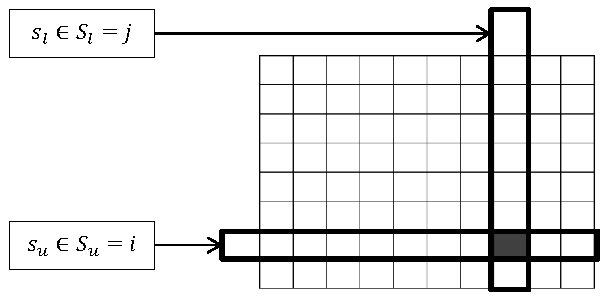
\includegraphics{media/figure7.pdf}
 

The first alteration that can be made, is to convert the problem into
multi-agent MDP; the problem is constructed of a parent MDP and a set of
independent children MDPs. The parent MDP's definition can be expanded
in the following manner:

\begin{itemize}
\item
  \(S_{u}  = X^{1},X^{n}\)
\item
  \(A_{u} = {\{ - 1, 0, 1\}}^{n}\)
\item
  \(\text{Transition}\)
\item
  \(R_{u}\left( u + a_{u}|a_{u}, u, E_{e} \right) = \sum_{i \in \{ 1,\ldots,n\}}R_{u,i}\left( s_{u,e + 1}|a_{u,e}, s_{u,e}, E_{e} \right)\)

  \begin{itemize}
  \item
    Noting
    \(R_{u,i}\left( s_{u,e + 1}|a_{u,e}, s_{u,e}, E_{e} \right) = \sum_{t \in E_{e}}^{\ }\frac{R_{l}\left( s_{l, t + 1}|a_{l,t}, s_{l,t}, s_{u,t} \right)}{\overline{\overline E}_{e}} - \sum_{t \in E_{e}^{o}}^{\ }\frac{R_{l}\left( s_{l,t + 1}|a_{l,t}, s_{l,t}, s_{u,t} \right)}{\overline{\overline E}_{e}^{o}}\)
  \end{itemize}
\end{itemize}

Expanding the state by a factor of \(n\) allows for the parent MDP to
regress to an optimal policy over \(\text{n\ }\)agents with an
exponential increase in both state space and action space. However, this
state space expansion is bounded by \(O(\left| X^{n} \right|)\) whereas
the multi-agent nMDP space space requirements are bounded by
\(O(\left| X^{n} \right|\left| X^{n} \right|n)\).

 
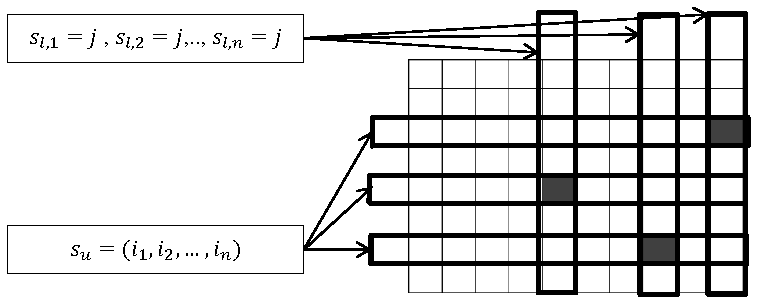
\includegraphics{media/figure8}
 


\subsubsection{Convergence}\label{convergence-1}

We can analyze policy convergence for both the \emph{multi-agent}
\emph{child} MDPs, and the \emph{multi-agent} \emph{parent} MDP: First,
the \emph{multi-agent child} MDPs remain unchanged, so given sufficient
policy execution time, their convergence is assured. Second, the
\emph{multi-agent} parent MDP converges similarly as shown in section 1:
The state space, action space, and transition space have increased in
dimension, which does not affect convergence{[}{]}. The Reward, although
now a sum over the agents, is a sum over a set of stably stochastic
functions, which is itself stably stochastic{[}{]}.

\subsubsection{complete multi-agent
CMDP}\label{complete-multi-agent-cmdp}

Thus, we can imagine the current problem as a search for the highest
cell numbers in a grid spread over number (\(n\)) of columns, where the
number of total columns is unlimited. It is natural, at this point, to
expand the \emph{multi-agent child} MDP into a \emph{complete
multi-agent child} MDP, by solving a two dimensional row problem:

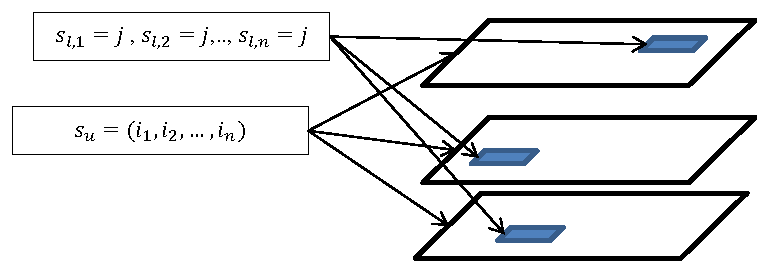
\includegraphics{media/figure9}
 
This division of space can be readily generalized to a foraging problem,
where each layer \(i\) is assigned reward such that reward increases as
a foraging targets location is nearer:

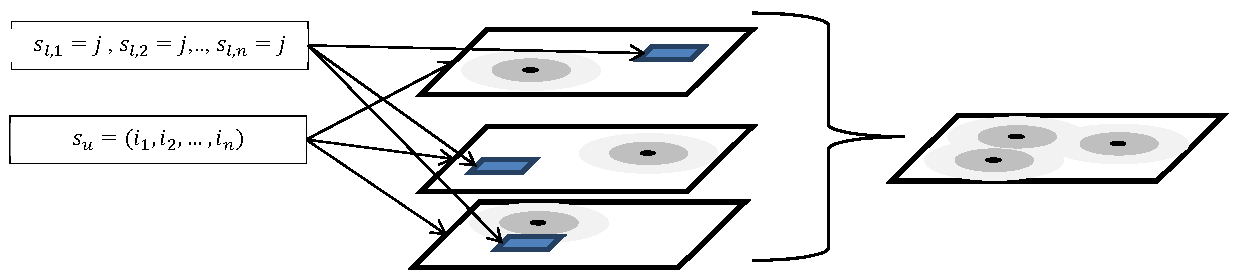
\includegraphics{media/figure10}

\subsubsection{}\label{section}

\subsubsection{Convergence}\label{convergence-2}

The complete model differs only in that state space is larger, and that
the model must contain a definition for a series of \(k\) sets,
\(k \in \left\{ X,X \right\}^{n}\). If we assume the \(k\) values set
for any experiment, we see that the only difference in models is that
the state space has increased in dimension. Aside from an increase in
computational and storage space burden, convergence in increased state
spaces is assured.

Thus, using this methodology, many general multi-agent problems can be
derived from the initial situation given within section 3.0, including
the assurance that, as time increased policy uncertainty asymptotically
decreases.

This remodelling, however, requires a human expert to complete. It may
be more enticing to consider how CMDP models may reconfigure dynamically
to solve problems, and how such models can be regularized. The remainder
of this paper considers how multiple approaches may be derived and
combined to create a general and regularized reinforcement learning
framework.

\section{General Reinforcement
Learning}\label{general-reinforcement-learning}

In the following section, the approach to finding a policy for a
singular MDP, \(M = \langle S, A, T, R \rangle \), is generalized; instead of relying on
a human to decide how to structure a CMDP, as described in sections 3.0
and 3.1, it may be desired that a reinforcement learning mechanism learn
its own structure. This learning mechanism is inspired by all domans of
research not limited to regularized neural networks and projected
component analysis{[}{]}. In both of these domains models learn
generative state space representations by initially (1) isolating
principal components that information can be projected onto and
following to (2) analyze and predict outcomes using the independent
subspaces noting covariance information. These methods sometimes do not
consider (3) the usage of information to make predictions of drive
actions of an agent within their environment. Thus, in the following
sections we construct a model that can automatically analyze the
components of state and action space, fulfilling (1) and (2), where this
method is tied to the performance of (3) the dynamic CMDP's ability to
both exhibit reduced space consumption and have increased decision
making and policy convergence behaviour.

The mechanism is formed using several sub behaviours. First, an nMDP can
be broken into a CMDP, which we know converges at time infinity. For
this decomposition and recomposition to be genrally applied, we need a
method to map Transitional and Policy information between similar
models. This is addressed in section 4.1 Learning and Mapping
Transitional Knowledge. Afterward, knowing that nMDP models and CMDP
models can be continually decomposed and recomposed, an approach to
expressing the decomposition/composition behaviour as a reinforcement
learning problem is expressed, in section 4.2 as Dynamic Reconfiguration
of Concurrent Markov Decision Processes.

\subsection{Learning and Usage of Transitional
Knowledge}\label{learning-and-usage-of-transitional-knowledge}

In this section we consider the benefits and drawbacks of modelling the
regressed Q values directly for a behavioural policy. The classic
initial approach is to discover \(Q\).
\begin{equation}
Q:\,S \times A \rightarrow \mathbb{R}^{+}
\end{equation}
Such that it is elementary to derive the behavioural policy online:
\begin{equation}
\pi^{*}:S \rightarrow A
\end{equation}

Where a common policy definition is commonly used in casual
experimentation, \(\pi^{*}(s) = \argmax_{a}Q(s,a)\).

The calculation of Q has been traditionally computed online using
equation (XX), repeated for reference:
\begin{equation}
{Q(s,a)}^{'} \leftarrow Q(s,a) + \alpha\left( R\left( s,a,s^{'} \right) - Q\left( s,a \right) + \max_{a^{*}}Q(s^{'},a^{*}) \right)
\end{equation}

Where the symbol (`) represents a function or variable value at the
following time step. The procedure of executing Q-Learning (\(Q_{l}\))
computes the a map,
\begin{equation}
Q_{l}:\,R(S,A,S) \times T(S,A,S) \rightarrow Q(S,A)
\end{equation}
, such that neither the complete reward (\(R(S,A,S)\)) or transition
(\(T(S,A,S)\)) images are kept in memory; the \(\text{QL}\) algorithm
functions \(\text{online}\). The purpose of this section is to, first,
provide a mechanism that stores and calculates Q values based on
learning approximate characterizing functions, for transition
\(\tilde{T}(S,A,S) \approx T(S,A,S)\) and reward
\(\tilde{R}\left( S,A,S \right) = R(S,A,S)\), by executing transition
learning and reward learning, \(T_{l},R_{l}\). Second, this section
outlines a method to recover Q values from these images anytime, using
\emph{transitional learning,} \(Q_{\text{tr}}\):
\begin{align}
%
T_{l}:&\,\tilde{T}\left( S,A,S \right) \times \left\{ \left( s,a,s^{'} \right) \right\} \rightarrow {\tilde{T}}^{'}(S,A,S)\notag\\
%
R_{l}:&\,\tilde{R}\left( S,A,S \right) \times \{(s,a,s^{'})\} \rightarrow {\tilde{R}}^{'}(S,A,S)\\
%
Q_{\text{tr}}:&\,{\tilde{T}(S,A,S)}^{'} \times {\tilde{R}(S,A,S)}^{'} \rightarrow Q^{'}(S,A)\notag
%
\end{align}
Thus, it is expected that the basis functions \(T_{l}\) and
\(R_{l}\ \)are computed online, whereas the current Q-Values can be
updated as needed using a process \(Q_{\text{tr}}\), to be outlined.

The \(T_{l}\) and \(R_{l}\) functions can be discovered, in the
following manner, through the tracking of local visitation frequencies:

 
\begin{equation*}
T_{l}:\ \tilde{T}'\left( s,a,s' \right) \leftarrow \tilde{T}\left( s,a,s' \right) + \alpha\left( \frac{\text{fr}\left( s,a,s^{'} \right) + 1}{\text{fr}\left( s,a \right) + 1} - \tilde{T}\left( s,a,s' \right) \right)
\end{equation*}
\begin{equation*}
\frac{\text{fr}\left( s,a,s^{'} \right) + 1}{\text{fr}\left( s,a \right) + 1} = \frac{1 + \ \tilde{T}\left( s,a,s' \right)}{1 + \ \sum_{s'}^{\ }{\tilde{T}\left( s,a,s' \right)}} 
\end{equation*}

The \(Q_{\text{tr}}\) function can be defined using one of three
regression functions, each with benefits and drawbacks, where \(\xi\)
represents a collection of sample states action state tuples,
\(\xi\left( s,a \right) \subseteq S \times A \times S\), where \(a\) and
\(b\) are constants:

\begin{itemize}
\item
  A greedy algorithm, which does not value any future reward.
\end{itemize}

\begin{equation}
Q^{'}(s,a) \leftarrow \frac{1}{\sum_{s'\  \in \ \xi(s,a)}^{\ }{\tilde{T}\left( s,a,s' \right)}}\sum_{s'\  \in \ \xi(s,a)}^{\ }{\tilde{T}\left( s,a,s' \right)\tilde{R}\left( s,a,s' \right)}
\end{equation} 

\begin{itemize}
\item
  A complete algorithm, which recursively explores potential for future
  reward:
\end{itemize}

 
\begin{equation}
Q^{'}(s,a) \leftarrow \frac{1}{\sum_{s'\  \in \ \xi(s,a)} {\tilde{T}\left( s,a,s' \right)}}\sum_{s'\  \in \ \xi(s,a)}^{\ }{\tilde{T}\left( s,a,s' \right)\tilde{R}\left( s,a,s' \right) + \gamma\max_{a^{*}}Q(s^{'},a^{*})}
\end{equation}

 

\begin{quote}
This approach is the most complete, but runs into issues related to
recursive state space explosion.
\end{quote}

\begin{itemize}
\item
  A monte carlo algorithm, which runs a batch monte carlo simulation to
  update policy values:
\end{itemize}
 
\begin{equation}
Q^{'}\left( s,a \right) \leftarrow Q^{\ }\left( s,a \right) + \ \frac{\alpha}{n}\sum_{i = 0}^{\text{n\ }}{\tilde{R}\left( s,a,s' \right) - Q \left( s,a \right) + \gamma\argmax_{a^{*}}{Q(s^{'},a^{*})}}
\end{equation}
 
, where \(s'\) is sampled from the density
\(\tilde{T}\left( s,a,s' \right)\). It is trivial to note that the monte
carlo simulation approaches the value obtained by the complete algorithm
as the limit of \(n\) approaches infinity.

Thus, using elementary techniques it is tractable to regress to
transitional and reward models online, and it is furher possible to
extract policy values online using at least three algorithms.

\subsection{Transferring Knowledge}\label{transferring-knowledge}

Given an nMDP, it may be desired to split or reformulate a problem into
a CMDP. In this circumstance, given transition and reward data encoded
in a manner according to section 4.1, the next step is to consider how a
knowledge transference model may be constructed. For the following
section we will generalize the notion of state action result sets to the
notion of trajectories such that
\(l_{i}^{j} = \left\{ (s_{i},a_{i},s_{i}^{'}) \right\}_{i}^{j}\).

Using this notation
\(\tilde{T}\left( s,a,s' \right) = P\left( s^{'}|s,a \right) = \tilde{T}\left( l_{i}^{i + 1} \right)\ \)where
\(l_{i}^{i + 1} = \left\{ (s_{i},a_{i},s_{i}^{'}) \right\}_{i}^{i + 1}\).
The value for a transition sequence is a set of values
\(\tilde{T}\left( l_{i}^{j} \right) = \left\{ \tilde{T}\left( l_{i}^{i} \right) \right\}_{i}^{j}\)
. Lastly, to simplify analysis, we define a function
\(\tilde{F}\  \in \{\tilde{T},\tilde{R}\}\). We also recall
\(m_{k} = < S_{k},A_{k},T_{k},R_{k},{\tilde{T}}_{k},{\tilde{R}}_{k},\pi_{k} >\).

\subsubsection{Preliminary Deconstruction and Reconstruction
}\label{preliminary-deconstruction-and-reconstruction}

The goal is to describe a deconstruction \(d_{x}^{\text{yz}}\)and
reconstruction \(c_{\text{yz}}^{x}\)function, which maintain all of the
properties outlined in sections 3.0. This section begins by using the
CMDP via a gating function and regression is discussed.

\subsubsubsection{Decision Making and
Gating}\label{decision-making-and-gating}

Before this, however, it is prudent to consider how a behaviour policy
\(\pi_{x}\) can be mapped from a degenerate behaviour policy set
\(\left\{ \pi_{y},\pi_{z} \right\}\). Simply, we allow for definition of
a surjective confidence function
\(g_{x}:S \times \ \pi_{y}(S) \times \pi_{z}(S) \rightarrow \mathbb{R}^{+}\).
Where, typically,
\(\pi_{x}\left( s,a \right) = \operatorname{}{g_{x}\left( s,\pi_{y}\left( s \right),\pi_{z}(s) \right)}\).
It seems obvious at this point to formulate this gating function as the
result of a reinforcement learning mechanism.

\subsubsubsection{Na\"{i}ve Deconstruction and
Reconstruction}\label{nauxefve-deconstruction-and-reconstruction}
 
\begin{equation}
d_{x}^{\text{yz}}:m_{x} \rightarrow \ \left\{ m_{y},m_{z}|\ S_{y} \times S_{z} = S_{x},\ A_{y} \cup A_{z} = A_{x},\ {\tilde{c}}_{\text{yz}}^{x}\left( {\tilde{d}}_{x}^{\text{yz}}\left( \tilde{F} \right) \right) = \left( \tilde{F} \right) \right\} 
\end{equation}

\begin{equation}
c_{x}^{\text{yz}}:\left\{ m_{y}, \right\} \rightarrow \ \left\{ m_{x}|\ S_{y} \times S_{z} = S_{x},\ A_{y} \cup A_{z} = A_{x},\ {\tilde{c}}_{\text{yz}}^{x}\left( {\tilde{d}}_{x}^{\text{yz}}\left( \tilde{F} \right) \right) = \left( \tilde{F} \right) \right\} 
\end{equation}

Thus, splitting and merging are invertible processes. Importantly, the
character and performance of any chosen reconstruction sets
\(\left\{ d_{x}^{\text{yz}},c_{\text{yz}}^{x} \right\}\) are not implied
by usage of the functions. It can be illuminating to define some entry
level deconstruction set implementations for an nMDP:

\subsubsubsubsection{Example Na\"{i}ve
Deconstruction}\label{example-nauxefve-deconstruction}

A deconstruction implementation is provided: \(d_{x}^{\text{yz}}\). It
is direct to see that this implementation of \(d_{x}^{\text{yz}}\)
satisfies the axioms given in section 3.0.

\begin{itemize}
\item
  State

  A set of degenerate state spaces \(\{ S_{y}\ ,S_{z}\}\) can be defined
  using principle component analysis on a parent state space \(S_{x}\) ,
  being careful to include all dimensions from \(S_{x}\) in either
  \(S_{y}\) or \(S_{z}\).
\item
  Action

  The action set \(\{ A_{y}\ ,A_{z}\}\) can each be formed using a
  random selection of actions from \(A_{z}\). If actions are missing, (
  \(\left\{ A_{y} \cup A_{z} \right\}\backslash\ A_{x} \neq \varnothing\ \)
  ,) then the missing actions can simply be added,
  \(A_{y} \leftarrow A_{y}\  \cup \left\{ A_{x}\backslash\left\{ A_{y} \cup A_{z} \right\} \right\}\).
\item
  Transition

  Note:
  \(P\left( \left\{ s_{z}^{'},s_{y}^{'} \right\}|\left\{ a_{z},a_{y} \right\},\left\{ s_{z},s_{y} \right\} \right) = P\left( s_{x}^{'}|a_{x},s_{x} \right)\)

  The parent transition function \({\tilde{T}}_{x}\) can be projected
  onto subspaces \({\tilde{T}}_{y}\) and \({\tilde{T}}_{z}\). It is
  direct to note through application of the chain rule that a
  probability density describing transition can be broken into sub
  constituent distributions\(\backslash n\)
  \(P\left( s_{x}^{'}|a_{x},s_{x} \right) = \ P\left( s_{y}^{'},s_{z}^{'}|a_{x},a_{y},s_{y},s_{z} \right)\).
  Thus, In our current notation this notion can be stated briefly:
\end{itemize}

 
\begin{equation}
{\tilde{T}}_{y}\left( s_{y}^{'}|s_{y}^{\ },a_{y} \right) = \ \sum_{s_{z}^{'}}^{\ }{\sum_{a_{z}}^{\ }{\sum_{s_{z}}^{\ }{{\tilde{T}}_{x}\left( \left\{ s_{y}^{'},s_{z}^{'} \right\}|\left\{ s_{y}^{\ },s_{z}^{\ } \right\},\left\{ a_{y},a_{z} \right\} \right)\frac{\pi_{x}\left( a_{y},a_{z}|s_{y},s_{z} \right)}{\sum_{a_{z}^{'}}^{\ }{\pi_{x}\left( a_{y},a_{z}^{'}|s_{y},s_{z} \right)}}}}}
\end{equation}
 

It is worth noting that if we split the MDPs according to section 3.0,
specifically such that one MDP is the parent and the other is the child,
then we can reuse the \emph{Convergent Factors Lemma(}appendix).
Specifically the transition functions simplify:

For the child, \(z\), the parent will always hold its action \(a_{z}\)
constant, rendering its behavioural policy irrelevant for the purposes
of projecting transitional probability.

 
\begin{equation}
{\tilde{T}}_{z}\left( s_{z}^{'}|s_{z}^{\ },a_{z},a_{y} \right) \leftarrow \ \sum_{s_{z}^{'}}^{\ }{{\tilde{T}}_{x}\left( \left\{ s_{y}^{'},s_{z}^{'} \right\}|\left\{ s_{y}^{\ },s_{z}^{\ } \right\},\left\{ a_{z} \right\},a_{y} \right)}
\end{equation} 

For the parent, \(y\), the transition model must take into account a
sequence of actions undertaken

 
\begin{equation}
{\tilde{T}}_{y}\left( s_{y}^{'}|s_{y}^{\ },a_{y} \right) = \ \sum_{s_{z}^{'}}^{\ }{\sum_{a_{z}}^{\ }{{\tilde{T}}_{x}\left( \left\{ s_{y}^{'},s_{z}^{'} \right\}|\left\{ s_{y}^{\ },s_{z}^{\ } \right\},\left\{ a_{y},a_{z} \right\} \right)\pi_{z}\left( a_{z}|s_{z} \right)}}
\end{equation}
 

\begin{itemize}
\item
  Reward
\item
  Policy
\end{itemize}

It becomes apparent that the degenerate policy
\(\pi_{y}\left( a_{y}|s_{y} \right)\) is unknown, and needs to be
inferred from the complete policy \(\pi_{x}\left( a_{x}|s_{x} \right)\).
Briefly a direct mapping can be considered which is a projection of
\(\pi_{x}\left( \bullet \right)\ \) onto
\(\pi_{y}\left( \bullet \right)\), where \(\sigma\) is a normalization
constant:

\begin{equation}
\pi_{x}\left( a_{y}|s_{y} \right) = \ \sigma\sum_{s_{z}^{'}}^{\ }{\sum_{s_{z}}^{\ }{\sum_{a_{z}}^{\ }{{\tilde{T}}_{x}\left( \left\{ s_{y}^{'},s_{z}^{'} \right\}|\left\{ s_{y}^{\ },s_{z}^{\ } \right\},\left\{ a_{y},a_{z} \right\} \right)\pi_{x}\left( \left\{ s_{y}^{\ },s_{z}^{\ } \right\}|\left\{ s_{y}^{\ },s_{z}^{\ } \right\} \right)}}}
\end{equation}
 

In essence, the degenerate policy image
\(\pi_{x}\left( A_{y}|S_{y} \right)\)becomes the expectation of the
parent policy \(\pi_{x}\left( A_{x}|A_{x} \right)\) weighted by the
transitional expectation, and this can be taken as the
\(\pi_{y}\left( a_{y}|s_{y} \right) = \ \pi_{x}\left( a_{y}|s_{y} \right)\).

After policy is initialized, the behavioural policy can be updated using
Q-Learning or any other mechanism.

 
\subsubsubsubsection{Example Na\"{i}ve
Reconstruction}\label{example-nauxefve-reconstruction}

A reconstruction implementation is provided: \(c_{x}^{\text{yz}}\). It
is direct to see that this implementation of \(c_{x}^{\text{yz}}\)
satisfies the axioms given in section 3.0.

Similar to deconstruction, reconstruction steps can be expressed
direction as a mapping of \(\left\langle S,A,T,R \right\rangle\) tuples:

\begin{itemize}
\item
  State
\item
  \(S_{x} = S_{y} \times S_{z}\)
\item
  Action
\item
  \(A_{x} = A_{y} \cup A_{z}\)
\item
  Transitional probability
\item
  Knowing \(s_{x}^{'} = \left\{ s_{y}^{'},s_{z}^{'} \right\}\)
\item
  \({\tilde{T}}_{x}\left( \left\{ s_{y}^{'},s_{z}^{'} \right\}|\left\{ s_{y}^{\ },s_{z}^{\ } \right\},a_{x} \right) = {\tilde{T}}_{y}\left( s_{y}^{'}|s_{y}^{\ },a_{x} \right){\tilde{T}}_{z}\left( s_{z}^{'}|s_{z}^{\ },a_{x} \right)\)
\item
  Reward
\item
\item
  Policy
\item
\end{itemize} 

\subsubsubsection{Concurrency and
re-mapping}\label{concurrency-and-re-mapping}

Given the state space savings given by a degenerate formulation, it may
be desired to only represent nMDPs in their degenerate formats. Thus, in
general,

\subsubsection{Compensation for temporal scale
difference}\label{compensation-for-temporal-scale-difference}

(page 88)

\subsubsection{Compensation for action space
factorization}\label{compensation-for-action-space-factorization}

\subsubsubsection{Compensation for action space
factorization}\label{compensation-for-action-space-factorization-1}

\section{}\label{section-1}

\section{Simulation}\label{simulation-1}

\subsection{Experiment Two}\label{experiment-two}

\section{Results}\label{results}

\section{Conclusion}\label{conclusion}

\section{References}\label{references}

\section{Appendix: Convergent Factors
Lemma}\label{appendix-convergent-factors-lemma}

Note

The set of optimal policies \(\Omega_{\ }^{*}\left( i,j \right)\) can be
expressed as a union of two independent policies,
\(\left( \Omega_{u}^{*}\left( j \right),\Omega_{l}^{*}\left( i|j \right) \right),\)
for problems in the presented CMDP's class. For this proof, \(i\) and
\(j\) are taken to be two subspaces \(S_{I},S_{J}\) within a parent
state space \(S\), such that a bijective function exists,
\(f_{s},:\ S_{I} \times S_{J} \rightarrow S.\) We assume separable
actions for with another bijective map,
\(f_{a}:\ A_{I} \times A_{J} \rightarrow A\). It's worth noting that in
practicality, transformations such as affine projections and arbitrary
component projections, can be considered. To begin we can consider the
set of all optimal actions that maximize expected future discounted
reward.

 
\begin{equation}
\Omega_{\ }^{*}(a) = \argmax_{a}\sum_{s' \in S\ }^{\ }{P\left( s'|s,a \right)\left( R\left( s,a,s' \right) + \gamma V\left( s' \right) \right)}
\end{equation}
 
The argument is that there exists a mapping from two optimal sub
policies onto this policy.

\begin{equation} 
f:\Omega_{u}^{*}\left( S_{u} \right) \times \Omega_{l}^{*}\left( S_{l} \right) \rightarrow \ {\tilde{\Omega}}_{\ }^{*}\left( S_{\ } \right):{\tilde{\Omega}}_{\ }^{*}\left( S_{\ } \right) \subseteq \Omega_{\ }^{*}\left( S_{\ } \right)
\end{equation}

For the following analysis, consultation of a visual grid can be
beneficial. To simplify notation, \(\left( i,j \right)\ \)is taken to
equal \(\text{ij}\), and actions
\(\left( a_{u},a_{l} \right) = \ a_{\text{ul}}\).

\begin{equation}
\Omega_{\ }^{*}(i,j) =  \argmax_{\left(a_{u},a_{l}\right)}\sum_{\left( i',j' \right) \in S\ }^{\ }{P\left( i'j'|ij,a_{\text{ul}} \right)\left( R\left( ij,a_{\text{ul}},i'j' \right) + \gamma V\left( i'j' \right) \right)}
\end{equation}

knowing
\(  \max_{\left(a_{u},a_{l}\right)}R\left( \left( i,j \right),\left( a_{u},a_{l} \right),\left( i',j' \right) \right) = \max_{\left(a_{u},a_{l}\right)}R\left( \left( i,j' \right),\left( a_{u},a_{l} \right),\left( i',j' \right) \right)\)
allows the expression to be altered with \(j'\), using the exchange
lemma.

\begin{equation}
 \Omega_{\ }^{*}(\left( i,j \right)) =  \argmax_{\left(a_{u},a_{l}\right)}\sum_{\left( i',j' \right) \in S\ }^{\ }{P\left( \left( i',j' \right)|\left( i,j \right),\left( a_{u},a_{l} \right) \right)\left( R\left( \left( i,j' \right),\left( a_{u},a_{l} \right),\left( i',j' \right) \right) + \gamma V\left( \left( i',j' \right) \right) \right)}
\end{equation}

It then becomes clear that the reward dependency can be expressed in
terms of \(R_{l}\ \)only:

\begin{equation}
\Omega^{*}(\left( i,j \right)) = \argmax_{\left(a_{u},a_{l}\right)} \sum_{\left( i',j' \right) \in S\ }^{\ }{P\left( \left( i',j' \right)|\left( i,j \right),\left( a_{u},a_{l} \right) \right)\left( R_{l}\left( j^{'}|a_{l},i',j \right) + \gamma V\left( \left( i',j' \right) \right) \right)}
\end{equation}

At this point, it is possible to note that the Transition function may
be decomposed
\(P\left( \left( i',j' \right)|\left( i,j \right),\left( a_{u},a_{l} \right) \right) = P\left( i'|a_{l},i \right)P\left( j'|a_{u},j \right)\).

\begin{equation} 
\Omega^{*}(\left( i,j \right)) = \argmax_{\left(a_{u},a_{l}\right)}\sum_{\left( i',j' \right) \in S\ }P\left( i'|a_{l},i \right)P\left( j'|a_{u},j \right)\left( R_{l}\left( j^{'}|a_{l},i',j \right) + \gamma V\left( \left( i',j' \right) \right) \right)
\end{equation} 

Leading to a summation decomposition:
\begin{equation}
\Omega^{*}(\left( i,j \right)) =  \argmax_{\left(a_{u},a_{l}\right)}\sum_{i' \in S\ }P\left( i'|a_{u},i \right)\left\lbrack \sum_{j' \in S}^{\ } P\left( i'|a_{l},i \right)\left( R_{l}\left( j^{'}|a_{l},i',j \right) + \gamma V\left( \left( i',j' \right) \right) \right) \right\rbrack  
\end{equation}

It is also possible to take the difference between two reward functions,
differentiated by \(i\) and \(i\)', to achieve a favourable formulation.
This addition is possible because our formulation is considering an
optimal action, \(\left( a_{u},a_{l} \right)\).
\begin{equation}
\Omega^{*}\left( i,j \right) =  \argmax_{\left(a_{u},a_{l}\right)}\sum_{i' \in S\ }P\left( j'|a_{u},j \right)\left\lbrack \sum_{j' \in S}P\left( i'|a_{l},i \right)\left( R_{l}\left( j^{'}|a_{l},i',j \right) - R_{l}\left( {j'}^{\ }|a_{l},i,j \right) + \gamma V\left( i',j' \right) - \gamma V\left( i',j \right) \right)  \right\rbrack
\end{equation}
And, an optimal decision policy can be substituted in for action
selection
\(\Omega^{*}\left( j \middle| i \right) =  \argmax_{\left(a_{u},a_{l}\right)}\sum_{j' \in S\ }P\left( j'|a_{l},j \right)\left( R\left( j,a_{l},j^{'}|i \right) + \gamma V\left( j^{'}|i \right) \right)\).

\begin{equation}
\Omega^{*}\left( i,j \right) =  \argmax_{\left(a_{u},a_{l}\right)}\sum_{i' \in S\ }P\left( i'|a_{u},i \right)\left\lbrack \sum_{j' \in S}^{\ }P\left( j'|\Omega_{\ }^{*}\left( j \middle| i \right),j \right)\left( R_{l}\left( j^{'}|\Omega_{\ }^{*}\left( j \middle| i \right),i',j \right) - R_{l}\left( j^{\ }|\Omega^{*}\left( j \middle| i \right),i,j' \right) + \gamma V\left( i',j' \right) - \gamma V\left( i',j \right) \right) \right\rbrack
\end{equation}

The formulation can now be radically generalized:
\begin{equation}
\Omega^{*}\left( i,j \right) =  \argmax_{\left(a_{u},a_{l}\right)}
\sum_{i' \in S} 
P\left( i'|a_{u}, i \right)
\left\lbrack R_{u}\left(  i^{'}|a_{u}, j, i \right)+ \gamma V\left( i' \right) \right\rbrack
\qquad\textrm{if\ }
a_{u} \in\Omega_{l}^{*}\left( j|i \right)
\end{equation}

From here it is direct to union the row selection policy:
\begin{equation}
\Omega^{*}\left( i,j \right) =   \sum_{i' \in S}
P\left( i'|a_{u}, i \right)\left\lbrack R_{u}\left( i^{'}|a_{u}, i \right) + \gamma V\left( i' \right) \right\rbrack \cup \left\lbrack \Omega_{l}^{*}\left( j|i \right) \right\rbrack
\qquad\textrm{if\ }a_{u} \in\Omega_{l}^{*}\left( j|i \right)
\end{equation}
And substitute a definition only dependent on independent policies.
 
\begin{equation}
\Omega^{*}\left( i,j \right) = \Omega_{u}^{*}\left( i \right) \cup \Omega_{l}^{*}\left( j|i \right)
\end{equation}
 
And, it follows directly that a specific and optimal global policy can
be expressed as every combination of optimal CMDP policies.
\begin{equation}
\pi^{*}\left( i,j \right) = \pi_{u}^{*}\left( i \right) \cup \pi_{l}^{*}\left( j|i \right)
\end{equation}

We also know that execution of the regular action policies will converge
on these optimal policies.

\begin{equation}
\pi\left( i,j \right) = \pi_{u}^{\ }\left( i \right) \cup \pi_{l}^{\ }\left( j|i \right)
\end{equation}

\end{document}
